\subsection{ระบบที่ใช้ช่วยในการพัฒนาหุ่นยนต์}
Robot Middleware เป็นกรอบการทำงาน(framework) ที่มีความยืดหยุ่นสำหรับการพัฒนาซอฟแวร์ที่เกี่ยวข้องกับหุ่นยนต์ โดยมีเครื่องมือที่ช่วยติดต่อสื่อสารระหว่างอุปกรณ์ต่าง ๆของหุ่นยนต์ Robot Middleware ส่วนใหญ่จะใช้การติดต่อสื่อสารผ่านระบบเครือข่ายเน็ตเวิร์ค ทำให้การสื่อสารในระบบพื้นฐานเป็นอิสระต่อกัน และสามารถติดต่อสื่อสารกันกับอุปกรณ์ที่อยู่ภายนอกผ่านเครือข่ายเดียวกันได้
ปัจจุบันมี Robot Middleware ที่ถูกพัฒนาขึ้นมาให้ใช้อยู่หลายตัวเช่น
Player Project: เป็นโปรเจคที่ใช้ในการสร้างซอฟแวร์เพื่อการศึกษาวิจัยที่มีความเกี่ยวข้องกับหุ่นยนต์และระบบเซนเซอร์
YARP: เป็น open source ที่เขียนด้วยภาษา C++ ในการเชื่อมต่อกับเซนเซอร์ หน่วยประมวลผล และตัวขับเคลื่อนของหุ่นยนต์
URBI: เป็น open source สำหรับพัฒนาแอพพลิเคชั่นที่เกี่ยวข้องกับหุ่นยนต์หรือระบบที่มีความซับซ้อน ใช้ภาษาพื้นฐานเป็นภาษา C++ ติดต่อสื่อสารได้ภายในเครือข่ายเดียวกันเท่านั้น (Local Network)
MIRO: เป็นกรอบการทำงานของหุ่นยนต์ที่เคลื่อนที่ได้โดยเขียนในลักษณะเป็น OOP
OpenRDK: เป็น open source สำหรับพัฒนาระบบที่มีความเป็นอิสระต่อกัน (Modules) สามารถใช้ช่องทางการติดต่อสื่อสารและหน่วยความจำร่วมกันได้
ROS: เป็นแหล่งรวมเครื่องมือที่ใช้พัฒนาซอฟแวร์หุ่นยนต์

\clearpage
\subsection{ระบบที่ใช้ในการจำลองการทำงานของหุ่นยนต์}
โปรแกรมจำลองการทำงานของหุ่นยนต์นั้นเป็นเครื่องมือที่สำคัญสำหรับนักหุ่นยนต์ การใช้โปรแกรมจำลองนั้นจะช่วยเพิ่มประสิทธิภาพในการทำงานหลายอย่าง เช่น ให้รู้ว่าหุ่นยนต์ที่ออกแบบนั้นสามารถทำงานได้อย่างที่ต้องการหรือไม่ กระบวนการคิดถูกต้องหรือไม่ โปรแกรมจำลองระบบส่วนใหญ่จะคำนวณพลวัตของหุ่นยนต์โดยใช้เครื่องมือคำนวณ open dynamics engine (ODE)
USARSim


รูปที่ 2.9 ผลลัพธ์จากการใช้โปรแกรม USARSim
USARSim เป็นโอเพนซอร์ซและเหมาะสำหรับทำหุ่นยนต์ประเภทกู้ภัยในซากเมือง โดยมีฐานการพัฒนามาจาก Unreal Tournament game engine ภายในโปรแกรมมีเครื่องมือสำหรับการทำงานวิจัย มีเซนเซอร์ของหุ่นยนต์ที่หลากหลาย เช่น เซนเซอร์รับภาพ หรือเซนเซอร์ตรวจความเคลื่อนไหว
MuRoSimF

รูปที่ 2.10 ผลลัพธ์จากโปรแกรม MuRoSimF
MuRoSimF ย่อมาจากคำว่า Multi-Robot Simulation Framework เป็นเครื่องมือที่ช่วยทำระบบจำลองจาก Darmstadt University โปรแกรมระบบจำลองนี้มีการใช้งานที่ง่าย เหมาะสำหรับหุ่นยนต์หลายประเภท เช่น หุ่นยนต์เคลื่อนที่ด้วยล้อ หุ่นยนต์สองขา หรือหุ่นยนต์หลายขา สามารถคำนวณพลวัตร และการขัดกันของก้านต่อต่าง ๆได้
Gazebo

รูปที่ 2.11 โปรแกรม Gazebo ที่กำลังจำลอง HR OS5 Humanoid Research Platform
Gazebo เป็นโปรแกรมจำลองการทำงานของหุ่นยนต์ ที่มีความสามารถในการคำนวณการเดินและการเคลื่อนที่ของหุ่นยนต์ที่สลับซับซ้อนได้ สามารถเห็นภาพกราฟฟิคของหุ่นยนต์ขณะทำงาน โดยผู้ใช้สามารถกำหนดค่าตัวแปรทางฟิสิกส์ต่าง ๆได้ เช่นน้ำหนัก ค่าความเฉื่อย แรงเสียดทานของข้อต่อ ทำให้การออกแบบหุ่นยนต์หรือทดลองโปรแกรมได้เหมือนกับโลกจริง มีแสง มีเงา และ พื้นผิวของวัตถุ และที่พิเศษคือสามารถสังเคราะห์ค่าของเซนเซอร์ เซนเซอร์พร้อมสัญญาณรบกวน ค่าระยะทาง แรงบิด และอื่นๆ คำนวณพลศาสตร์ของหุ่นยนต์โดยใช้ตัวคำนวณทางฟิสิกส์เป็น Bullet หรือ Simbody ในการจำลองหุ่นยนต์ในโปรแกรมนี้จำเป็นต้องได้รับไฟล์ข้อมูลของหุ่นยนต์มาก่อนซึ่งอยู่ในรูปแบบของ URDF ซึ่ง URDF คือ ประเภทของไฟล์ที่บ่งบอกถึงความสัมพันธ์ของข้อต่อและก้านต่อแต่ละชิ้นในตัวหุ่นยนต์ มีความสามารถในการอธิบายถึงกลศาสตร์และการเคลื่อนที่ของหุ่นยนต์ รวมถึงตรวจสอบการขัดกันของก้านต่อในหุ่นยนต์ได้ ภายในไฟล์นี้จะประกอบไปด้วย
Link: คือก้านต่อของหุ่นยนต์ซึ่งภายในจะสามารถบอกขนาด รูปร่าง สี และสามารถ import 3d mesh เข้ามาได้ด้วย อีกทั้งยังสามารถใส่รายละเอียดของการเคลื่อนที่ ของก้านต่อได้เช่น inertial matrix และ collision properties
Joint: คือข้อต่อของหุ่นยนต์สามารถกำหนดกลศาสตร์และการเคลื่อนที่ได้เช่น Joint limits ของข้อต่อที่กำลังหมุนและความเร็วการหมุน ซึ่งข้อต่อมีหลายแบบที่สามารถกำหนดได้เช่น ข้อต่อแบบหมุน, ข้อต่อแบบเลื่อน, ข้อต้อต่อแบบยึดติด, ข้อต่อแบบต่อเนื่อง

\clearpage
\subsection{Robot Operating System}
Robot Operating System หรือ ROS ถูกพัฒนาโดยบริษัท Willow Garage, แต่เดิมแล้วเค้าพัฒนาเพื่อใช้งานกับหุ่นยนต์ PR2 ในปี 2007
ซึ่งพัฒนาเป็น open source framework สำหรับนักพัฒนาซอฟแวร์ที่เกี่ยวข้องกับหุ่นยนต์ มีความสามารถในการทำงานแบบ parallel
บนคอมพิวเตอร์หลายๆเครื่องได้ สามารถทำงานได้หลาย OS แต่ที่ซัพพอร์ทจริงๆคือ Ubuntu และ Debian นอกจากนี้ยังมีคลังที่คอยเก็บซอฟแวร์ต่างๆไว้เป็น
libraries อีกด้วย การใช้ ROS จะช่วยทำให้เราสามารถพัฒนาหุ่นยนต์ได้อย่างรวดเร็วมากขึ้น ประหยัดเวลา ประหยัดทรัพยากร
ในส่วนนี้จะกล่าวถึง ROS คร่าวๆ

\subsubsection*{Nodes}
Node เป็นเหมือนหน่วยประมวลผลในระบบ ROS, Node สามารถที่จะส่งข้อมูลหาโหนดอื่นๆได้ ผ่าน Topics หรือ Services
ในทางปฏิบัติแล้วโหนดเป็นตัวประมวลผลย่อยๆ ที่คอยทำหน้าที่เฉพาะ ยกตัวอย่างเช่น โหนดตัวแรกเชื่อมต่อกับกล้อง
เพื่อที่จะนำภาพจากกล้องออกมา โหนดตัวที่สองใช้ในการหาลูกบอลที่อยู่ในภาพที่ได้มาจากโหนดตัวแรก และโหนดตัวที่สามใช้ในการคำนวณหาตำแหน่งของลูกบอลที่อยู่บนโลกจริงๆ
จากตำแหน่งของลูกบอลที่ได้มาจากโหนดที่สอง ดังนั้นจะเห็นว่าแต่ละโหนดจะทำงานเฉพาะของตัวเอง ซึ่งสามารถนำมารวมกันได้ การเขียนเป็นแบบโหนดจะช่วยทำให้เราสามารถที่จะนำโปรแกรมกลับมา
แก้ไขปรับปรุงให้ใช้ใหม่ได้ง่าย ในกรณีที่จะนำไปทำงานอย่างอื่น ยกตัวอย่างเช่น โหนดที่เอาภาพจากกล้องออกมา อาจจะมีโหนดอีกตัว ทำหน้าที่ในการหาโกลด์เป้าหมาย และหาทิศทางการเคลื่อนที่ของหุ่นยนต์ได้
ดังนั้นการพัฒนาโหนดเป็นส่วนย่อยๆเล็กๆ ก็เพื่อที่จะทำให้การแก้ไขหรือปรับปรุงได้ง่าย
\begin{figure}[htbp]
	\centering	    
	\begin{tikzpicture}[shorten > = 1pt,scale=0.9, transform shape]
		% Place nodes
		\node [node] (image_provider) {image\_provider};
		\node [topic, below of=image_provider] (/image) {/image\\sensor\_msgs/Image.msg};
		\node [node, below left of=/image] (line_detection) {line\_detection};
		\node [node, below right of=/image] (stop_detection) {stop\_detection};
		\node [topic, below of=line_detection,xshift=-0.5cm] (/line) {/line\\example\_msgs/Line.msg};
		\node [topic, below of=stop_detection,xshift=0.5cm] (/stop) {/stop\\example\_msgs/Stop.msg};
		\node [node, below of=/image, yshift=-3.0cm] (navigation) {navigation};
		\node [topic, below of=navigation] (/cmd_vel) {/cmd\_vel\\geometry\_msgs/Twist.msg};
		\node [node, below of=/cmd_vel,yshift=1cm] (robot_control) {robot\_control};
		% % Draw edges
		\path [line] (image_provider) -- (/image);
		\path [line] (/image) -- (line_detection);
		\path [line] (/image) -- (stop_detection);
		\path [line] (line_detection) -- (/line);
		\path [line] (stop_detection) -- (/stop);
		\path [line] (/line) -- (navigation);
		\path [line] (/stop) -- (navigation);
		\path [line] (navigation) -- (/cmd_vel);
		\path [line] (/cmd_vel) -- (robot_control);
	\end{tikzpicture}
	\caption{ตัวอย่างสถาปัตยกรรมของ ROS}
	\label{fig:ros_architecture}
\end{figure}

จากตัวอย่างสถาปัตยกรรมของ ROS ดังรูปที่ \ref{fig:ros_architecture} นั้นสามารถอธิบายได้ว่า หุ่นยนต์เคลื่อนที่ด้วยล้อมีภารกิจคือ
เคลื่อนที่ตามเส้นไปเรื่อยๆจนกว่าจะเจอเครื่องหมายหยุด Node คือตัวที่แสดงด้วยรูปวงรี ข้างในเป็นชื่อโหนด ส่วน Topic จะแสดงด้วยรูปสี่เหลี่ยม
ซึ่งข้างในเป็นชื่อของ Topic และชนิดของ Message ที่ใช้ในการส่งข้อมูล, มาดูกันก่อนอื่น ภาพถูกส่งมาจากกล้อง และก็มีโหนดสองตัวในการดูเส้น และเครื่องหมายหยุด
จากภาพที่ได้มา เมื่อโหนดได้ข้อมูลแล้วก็นำมาประมวลผลการเดินของหุ่นยนต์โดยส่งไปยัง node navigation และโหนดนี้ก็จะทำหน้าที่คำนวณความเร็วและทิศทางของหุ่นยนต์
ส่งไปยัง node robot\_control ซึ่งเป็นตัวสั่งการมอเตอร์ของหุ่นยนต์อีกทีนึง
\begin{table}[htbp]
	\begin{subtable}[h]{0.40\textwidth}
		\centering
		\begin{tabular}{| p{4cm}| p{1.5cm} |}
			\hline 
			\multicolumn{2}{|c|}{Twist.msg} \\
			\hline
			geometry\_msgs/Vector3 & linear  \\
			geometry\_msgs/Vector3 & angular \\
			\hline  
		\end{tabular}
		\caption{Message Twist}
		\label{tab:message_twist}
	\end{subtable}
	\hfill
	\begin{subtable}[h]{0.40\textwidth}
		\centering
		\begin{tabular}{| p{1.5cm}| p{2.5cm} |}
			\hline 
			\multicolumn{2}{|c|}{Stop.msg} \\
			\hline
			uint8   & RED = 0   \\
			uint8   & GREEN = 1 \\
			uint8   & color     \\
			float32 & distance  \\
			\hline  
		\end{tabular}
		\caption{Message Stop}
		\label{tab:message_stop}
	\end{subtable}
	\caption{ตัวอย่างชื่อและข้อมูลของ Message}
	\label{tab:message_example}
\end{table}

ตัวอย่างของ Message สองอันนี้ Twist message (รูปที่ \ref{tab:message_twist}) คือ message ที่เอาไว้บอกความเร็วเชิงเส้น และความเร็วเชิงมุม
ซึ่ง ROS มี message ชนิดนี้ให้อยู่แล้ว ส่วน Stop message (รูปที่ \ref{tab:message_stop}) คือ message ที่เอาไว้บอกระยะทางและสีของป้าย Stop
ซึ่ง message นี้ถูกสร้างขึ้นมาใหม่เพื่อใช้กับงานนี้โดยเฉพาะ ดังรูปที่ \ref{fig:ros_architecture}

\subsubsection*{Topics and Messages}
Messages เป็นตัวหลักสำคัญในการติดต่อสื่อสารกันระหว่างโหนดใน ROS โดยที่ message จะถูกส่งผ่านไปยัง topic เสมอ
และ topic จะต้องมีที่เฉพาะ แต่ละ topic จะใช้ชนิดของ message เป็นอันเดียว 

Messages are the main communication method between ROS nodes.  Messages are
always published on a topic, which is identified by a name and can only transmit
one  type  of  message.   A  node  can  subscribe  to  a  topic  and  will  get  the  messages
other nodes publish to it.  Each node can subscribe to and publish on any number
of topics and will not know with whom it communicates.
Communication can happen between nodes running on the same computer as well
as nodes distributed over different computers,  as long as they are connected with
an TCP/IP network.  This is not only useful for parallelization but also eases the
visualization of the robots state on a separate desktop computer.  Each message has
a type which is either predefined in the ROS system or defined by a user package.
The interface of a node is mainly defined by the types of the messages it subscribes
and publishes.  These types can be either predefined in ROS or be newly created by
a developer, cp.  figure 2.5.

\subsubsection*{roscore}
The
roscore
is the most central part of a running ROS system.  It consists of the
rosmaster
,  the  ROS  parameter  server  and  the
rosout
logging  node.   The  ROS
master is registering which topics are published by the nodes and on which topics
nodes want to subscribe.  If one node wants to subscribe to a topic which another
node is publishing,  a peer-to-peer connection is established from one node to the
other.  Thereby the master does not become a bottleneck since it only connects the
nodes but does not need to handle the messages.  To do this, a subscribing node asks
the master for a list of nodes which publish on this named topic.  The master holds
a  table  of  all  publishers  and  sends  their  names  to  the  subscribing  nodes.   It  also
remembers which nodes are subscribing to this topic, if a new publisher is started
later.  This process is shown in figure 2.6.
The ROS parameter server is a global key-value store.  It is mainly designed to
be  used  for  static  configuration  parameters.   Transmission  of  data  between  nodes
should be done via topics to prevent making the parameter server a bottleneck.  All
parameters are globally visible.  If a parameter should be able to be changed during
runtime,  dynamic reconfigure can be used.  It provides the possibility to state on
compile  time  which  parameter  values  should  be  changeable  and  provides  an
rqt
plug-in for it, see section 2.3.9.  The
rosout
logging node subscribes to the
/rosout
topic which is the standard topic for logging.  ROS has built in methods to send
data to this topic which are displayed on runtime and written in a log file

\subsubsection*{Services}
Services  can  be  seen  as  remote  procedure  calls  (RPC).  In  contrast  to  messages
which are an unidirectional stream of data,  service calls are blocking and waiting
for a response.  They have defined types which consist of a request and a response
message.  The node providing the service is called server and the node calling the
service  is  called  client.   Services  are  useful  for  fast  tasks,  but  should  not  be  used
when getting the result can take a long time,  because the calling node is blocked
until completion.  For longer tasks, actions should be used (section 2.3.5).  A possible
service for the example described in figure 2.4 would be a manual stop service.  It
would be advertised by the navigation node and would stop the robot even without
markers.  As this would take not a lot of time, basically just alternating the state of
the navigation node, this would be possible to do with a blocking service call.

\subsubsection*{Actions}
Actions  are  used  when  a  task  which  takes  a  long  time  should  be  called  asyn-
chronously, in contrast to the synchronous service calls.  Each action has a specified
type which consists of three messages:  goal, feedback, and result.  A node providing
the action, the action server, is called by another node, the action client, by sending
a goal.  The action server will now try to achieve this goal, while the action client is
not blocked and can perform other tasks.  The server will constantly send feedback
messages to the client to inform it about the status of the process towards the goal.
The server will send a result message when the goal was reached or if the action was
interrupted.  Actions can be interrupted by sending new goals which the server con-
siders more important or by request of the action client, for example, if the sent goal
is not useful anymore.  A possible action for the example described in 2.4 would be
driving a certain distance on the line.  This needs some time because the robot has
to move.  Therefore a blocking call is not feasible.  The action runs asynchronously
and can also be interrupted, for example, if the line ends before reaching the desired
distance.

\subsubsection*{Code Organization}
The smallest and main unit for organizing software for ROS is a package.  A package
has a
package.xml
\ref{fig:example_packagexml} which describes different metadata of this package,
e.g.  the package name, the author, the license and dependencies on other packages.
A package can build on its own if all dependencies are met.  The content can, among
other things, be ROS nodes, visualization plug ins, libraries or datasets.  It can be
distinguished between dependencies on build and runtime.  Different packages can
be grouped in meta-packages, which hold no content of their own but only collect
packages which belong together.

\begin{figure}[htbp]
    \centering
    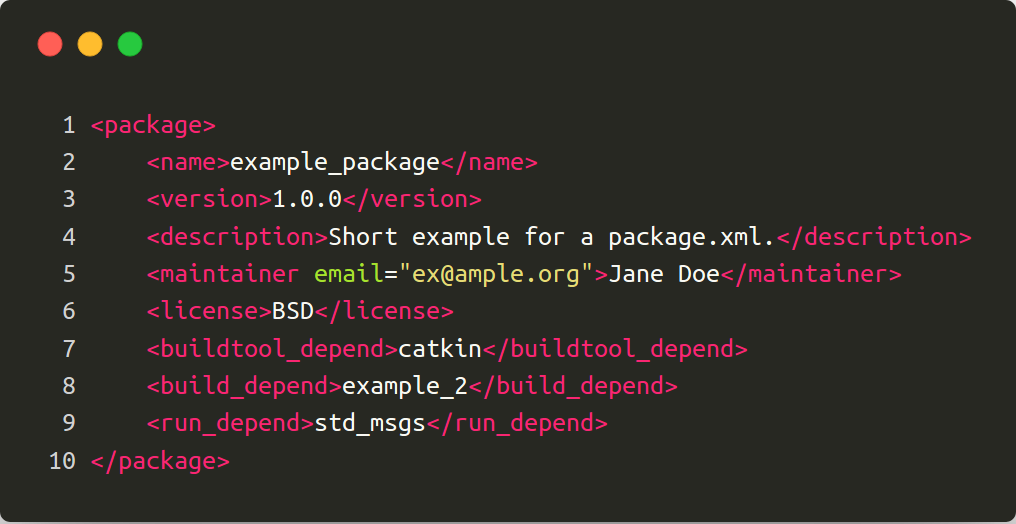
\includegraphics[width=0.8\textwidth]{chapter2/images/example_packagexml.png}
	\caption{ตัวอย่างไฟล์ package.xml แต่ละ tags สามารถใช้ในการบอกข้อมูลของ package นี้
	ใครเป็นเจ้าของ ใครเป็นคนเขียน รวมไปถึง dependencies ที่จำเป็นต้องใช้ของ package นี้ด้วย}
    \label{fig:example_packagexml}
\end{figure}

\subsubsection*{Code Distribution}
การที่จะนำ Nodes กลับมาใช้ใหม่หรือเอาออกมาแชร์ได้นั้น จะต้องมีการทำเอกสารของ Packages นั้นๆด้วย
โดยปกติแล้วจะถูกนำไปเก็บไว้ที่ GitHub และ package dependencies จะบอกไว้ในไฟล์ package.xml
เรียบร้อยแล้ว เพื่อให้ง่ายต่อการนำไปติดตั้ง หากผู้ที่นำไปใช้พัฒนาต่อหรือแก้ไขข้อผิดพลาดก็สามารถที่จะช่วยกันได้
โดยการ Pull request หรือ Report issues ได้

\subsubsection*{ROS Packages ที่ใช้ในงานวิจัย}
ในส่วนนี้จะอธิบายคร่าวๆถึง ROS standard packages ที่จะเอามาใช้ในงานวิจัยครั้งนี้
\paragraph*{rosbag}
rosbag เป็นแพกเกจที่สามารถบันทึก message ที่ส่งหากันในระหว่างที่ ROS กำลังทำงานได้
ไฟล์ที่บันทึกจะเรียกว่า rosbag ประโยชน์ของมันคือเราสามารถเอาเข้ามาใช้ในการตรวจสอบ
หรือนำมาเล่นซ้ำได้ อีกทั้งยังง่ายต่อการค้นหาข้อผิดพลาดอีกด้วย

\paragraph*{tf2}
tf2 เป็นแพกเกจที่สามารถติดตามการเปลี่ยนแปลงของ Coordinate frame เราสามารถใช้ในการหาความสัมพันธ์ระหว่าง
frame ได้ ยกตัวอย่างเช่นหากเราต้องการหาตำแหน่งของ foot เทียบกับ pelvis ก็สามารถใช้ tf2 หาได้

robot\_state\_publisher แพกเกจที่ subscribe JointState message เพื่อที่จะนำตำแหน่งของของข้อต่อ
และแปลงให้อยู่ในรูปข้อมูลของ tf2, tf2 สามารถเรียกจาก Node ใดๆก็ได้เพื่อที่จะหา Coordinate frame ที่ต้องการได้

\paragraph*{URDF}
Unified Robot Description Format (URDF) เป็นไฟล์ XML ที่เอาไว้อธิบายลักษณะของหุ่นยนต์
ใน ROS มีแพกเกจที่ใช้สำหรับการอ่านไฟล์ คือ urdf\_parser แต่ไฟล์นี้ก็มีการใช้งานโดย tf2 เช่นกัน

\paragraph*{xacro}
xacro เป็นไฟล์ XML เช่นเดียวกับ URDF โดยไฟล์ xacro นี้มีประโยชน์มากในการใช้งานใน ROS เพราะว่าทำให้การเขียนไฟล์
URDF ง่ายขึ้น เพราะสามารถทำเป็นมาโครได้ สามารถปรับแต่งค่าตัวแปรต่างๆได้ง่ายขึ้น

\subsubsection*{Visualization}
One of ROS’ core strengths is providing different tools for visualization.  Due to its
publisher-subscriber architecture, it is very easy to establish a data stream from the
program to the visualization.  Either the visualization can subscribe on topics that
are already being in use or additional topics can be provided from the software to
deliver more information to the visualization.  Messages in ROS are only published
if there is a subscriber on the topic, therefore publishing additional topics for visu-
alization reasons does not cost performance when the visualization is not running.
ROS provides two main tools for visualization which can be extended by plug-ins.
It is also possible to implement own tools which are independent from these.

\paragraph*{rqt}
rqt  is  a  QT  based  interface  with  ROS  connection \ref{fig:ros_gui_example}   Plug-ins  can  be
launched and provide a
QtWidget
.  Multiple widgets can be displayed at the same
time.  They can be resized and positioned by drag and drop.  ROS provides a set
of plug-ins but writing an own plug-in is possible too.  These plug-ins can be used
to visualize data in 2D but also to provide a controlling interface.  In the following,
some examples of important plug-ins are shown.
The
node
graph
plug-in shows all currently running nodes and topics.  Published
and subscribed topics are connected to their nodes and thereby it is easy to see the
flow of data.  This plug-in is especially helpful to get an overview of the running
software and to find misconnected nodes.
The
topic
monitor
lists all current topics.  It is possible to subscribe to them and
to get the current transmitted values.  Further on, statistics about the publishing
rate and the used bandwidth can be shown for each topic.
The
rqt
plot
plug-in  enables  live  plotting  of  data,  using
matplotlib
.    The
dynamic
reconfigure
plug-in provides an interface to change parameter values pre-
viously defined to be reconfigurable.  This is useful when tuning parameter values,
because  changing  it  is  possible  on  the  fly  and  does  not  require  a  restart  of  the
software


\begin{figure}[htbp]
    \centering
    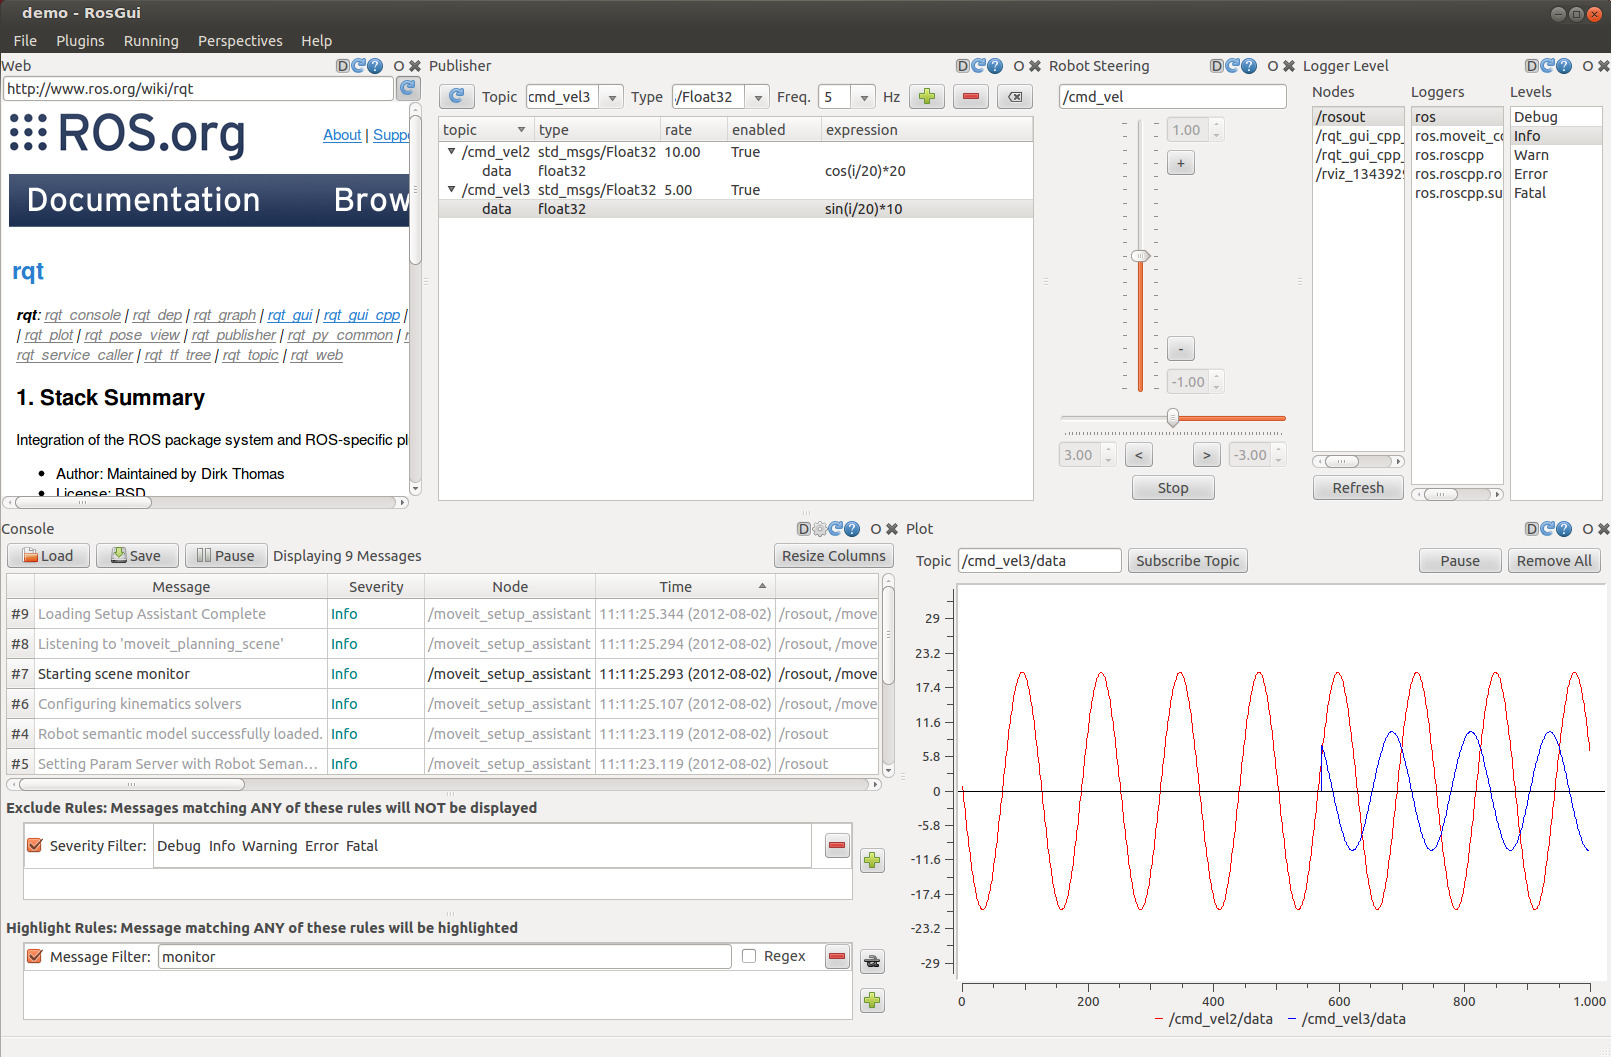
\includegraphics[width=0.8\textwidth]{chapter2/images/ros_gui_example.png}
	\caption{ตัวอย่างการแสดงผลใน rqt ในรูปเป็นการนำ rqt มาเขียนเป็น GUI ให้ผู้ใช้สามารถใช้งานได้ง่าย
	และสามารถที่จะปรับแต่ง parameters ต่างๆได้เรียลไทม์}
    \label{fig:ros_gui_example}
\end{figure}

\paragraph*{RViz}
RViz  provides  a  3D  visualization  of  the  robots  state  and  its  environment.   The
standardized URDF format is used to get a visual robot model, which is then used
to  show  the  current  positions  of  the  robots  joints.   Furthermore,  sensor  data  can
be displayed using marker messages.  These messages can be published by any node
and define three dimensional states which are displayed in RViz.  This is for example
helpful to get a visualization of recognized objects.  Furthermore, a lot of different
standard  ROS  messages  can  directly  be  visualized  in  RViz,  e.g.   camera  images,
depth  clouds,  laser  scans  and  point  clouds.   Thereby  RViz  provides  visualization
without additional effort, if the standard messages are used.  It is especially used for
localization and mapping, because it is possible to see the current sensor inputs of
the robot as well as its map in the same window \ref{fig:example_visualization_rviz}

\begin{figure}[htbp]
    \centering
    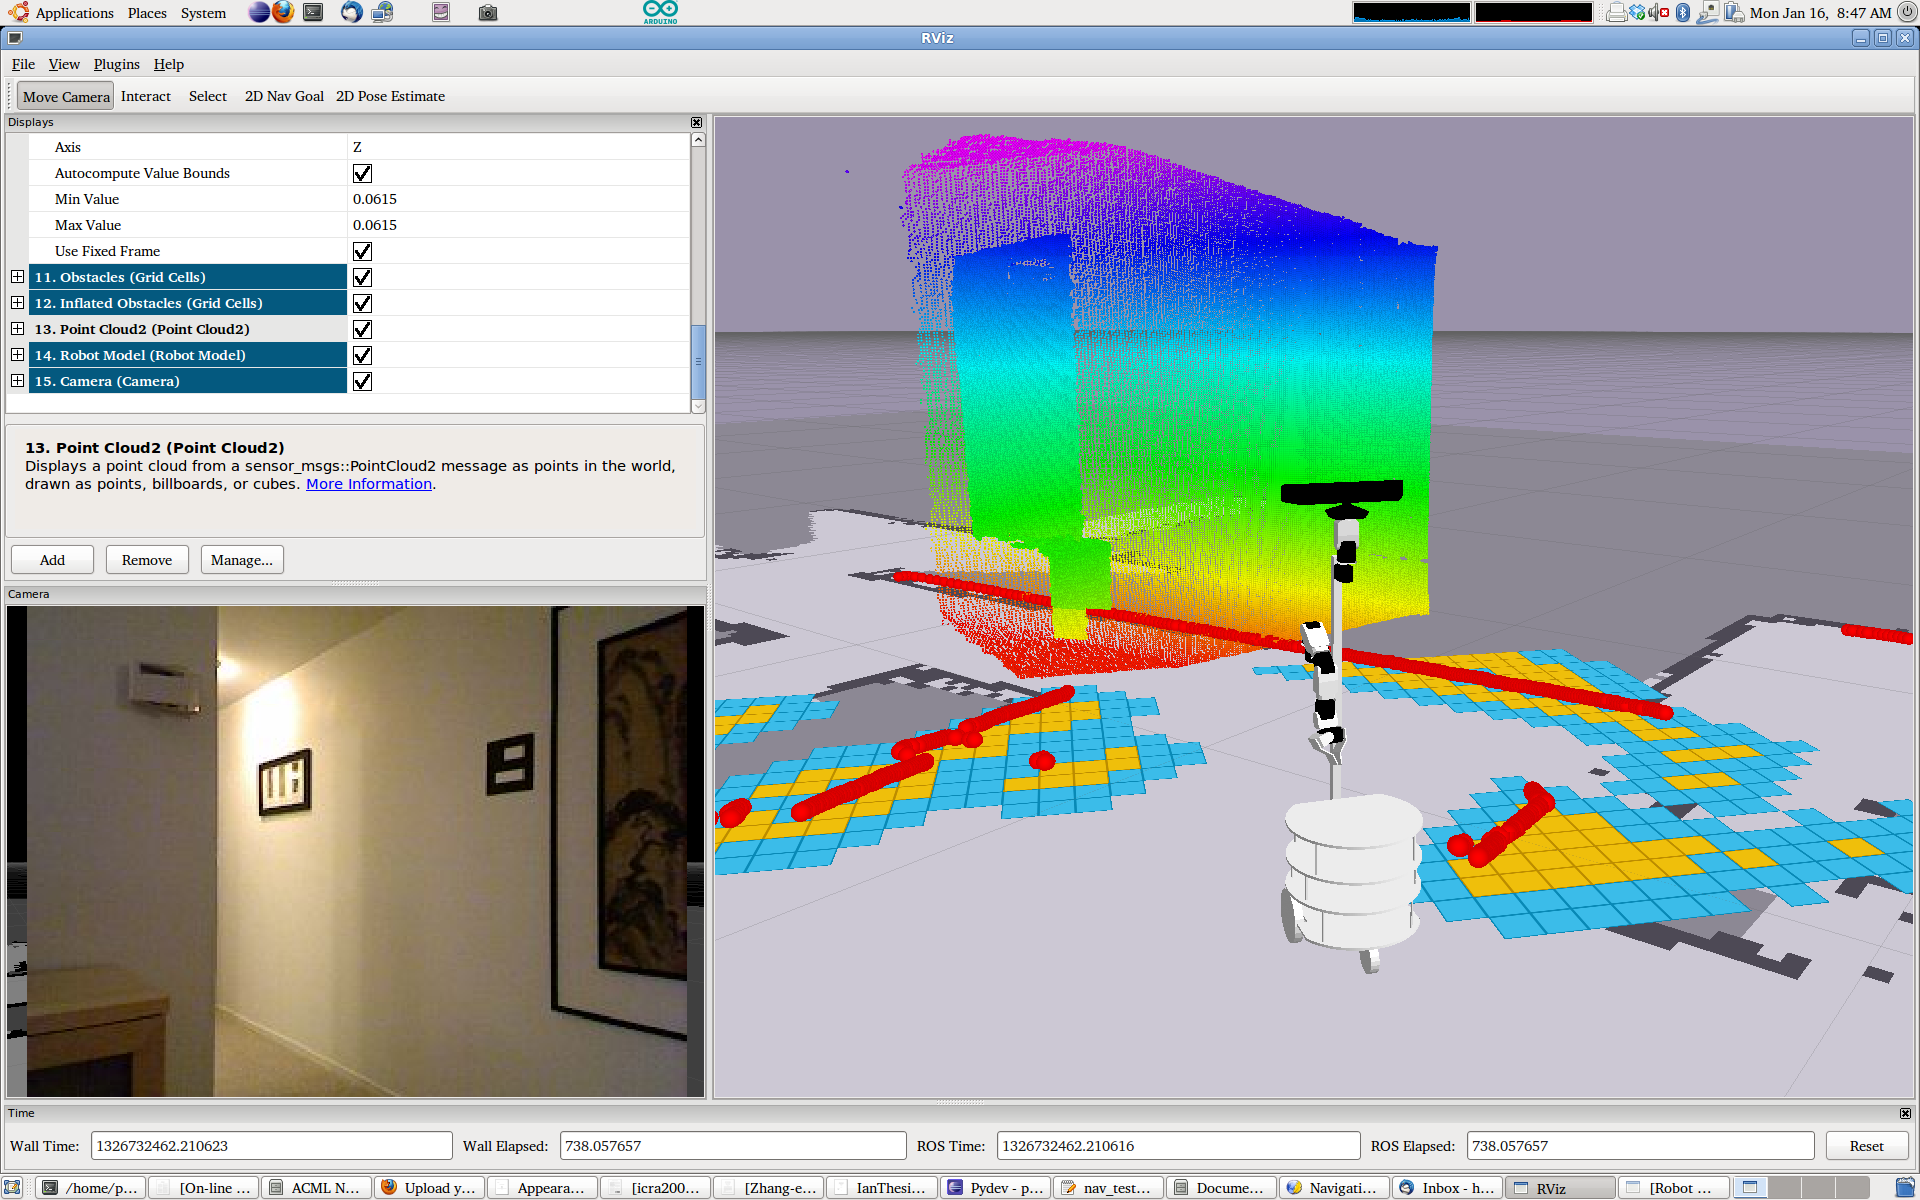
\includegraphics[width=0.8\textwidth]{chapter2/images/nav_test_rviz_2.png}
	\caption{ตัวอย่างการแสดงผลใน RViz ในรูปนี้เป็นเคสของหุ่นยนต์เคลื่อนที่ด้วยล้อ และทำแผนที่ด้วยข้อมูลความลึกที่ได้มาจาก Kinect}
    \label{fig:example_visualization_rviz}
\end{figure}



\subsubsection*{Simulation}
Simulation is a crucial part when developing robot software, since it gives the devel-
oper the possibility to run his software without using hardware.  This can prevent
hardware damages because bugs can be found before running it on the robot and
it can be used to accelerate development, e.g.  by testing in faster than real time.
While ROS can generally use any simulator, Gazebo is normally preferred, since it
has a good ROS integration and was also originally developed for ROS. In order to
use Gazebo, an URDF of the robot is required.
This  URDF  is  used  to  display  the  robot  in  the  simulator  and  to  compute  its
collisions with itself and the environment.  The simulator can provide sensor data
in  the  corresponding  standard  messages.   To  actuate  the  servos  of  the  robot,  dif-
ferent  controllers  are  available  which  work  with  the  corresponding  messages,  e.g.
JointTrajectory
